\PassOptionsToPackage{unicode=true}{hyperref} % options for packages loaded elsewhere
\PassOptionsToPackage{hyphens}{url}
%
\documentclass[]{book}
\usepackage{lmodern}
\usepackage{amssymb,amsmath}
\usepackage{ifxetex,ifluatex}
\usepackage{fixltx2e} % provides \textsubscript
\ifnum 0\ifxetex 1\fi\ifluatex 1\fi=0 % if pdftex
  \usepackage[T1]{fontenc}
  \usepackage[utf8]{inputenc}
  \usepackage{textcomp} % provides euro and other symbols
\else % if luatex or xelatex
  \usepackage{unicode-math}
  \defaultfontfeatures{Ligatures=TeX,Scale=MatchLowercase}
\fi
% use upquote if available, for straight quotes in verbatim environments
\IfFileExists{upquote.sty}{\usepackage{upquote}}{}
% use microtype if available
\IfFileExists{microtype.sty}{%
\usepackage[]{microtype}
\UseMicrotypeSet[protrusion]{basicmath} % disable protrusion for tt fonts
}{}
\IfFileExists{parskip.sty}{%
\usepackage{parskip}
}{% else
\setlength{\parindent}{0pt}
\setlength{\parskip}{6pt plus 2pt minus 1pt}
}
\usepackage{hyperref}
\hypersetup{
            pdftitle={Behind the Data: A Curated Set of Arctic Datasets},
            pdfborder={0 0 0},
            breaklinks=true}
\urlstyle{same}  % don't use monospace font for urls
\usepackage{longtable,booktabs}
% Fix footnotes in tables (requires footnote package)
\IfFileExists{footnote.sty}{\usepackage{footnote}\makesavenoteenv{longtable}}{}
\usepackage{graphicx,grffile}
\makeatletter
\def\maxwidth{\ifdim\Gin@nat@width>\linewidth\linewidth\else\Gin@nat@width\fi}
\def\maxheight{\ifdim\Gin@nat@height>\textheight\textheight\else\Gin@nat@height\fi}
\makeatother
% Scale images if necessary, so that they will not overflow the page
% margins by default, and it is still possible to overwrite the defaults
% using explicit options in \includegraphics[width, height, ...]{}
\setkeys{Gin}{width=\maxwidth,height=\maxheight,keepaspectratio}
\setlength{\emergencystretch}{3em}  % prevent overfull lines
\providecommand{\tightlist}{%
  \setlength{\itemsep}{0pt}\setlength{\parskip}{0pt}}
\setcounter{secnumdepth}{5}
% Redefines (sub)paragraphs to behave more like sections
\ifx\paragraph\undefined\else
\let\oldparagraph\paragraph
\renewcommand{\paragraph}[1]{\oldparagraph{#1}\mbox{}}
\fi
\ifx\subparagraph\undefined\else
\let\oldsubparagraph\subparagraph
\renewcommand{\subparagraph}[1]{\oldsubparagraph{#1}\mbox{}}
\fi

% set default figure placement to htbp
\makeatletter
\def\fps@figure{htbp}
\makeatother

\usepackage{booktabs}
\usepackage[]{natbib}
\bibliographystyle{apalike}

\title{Behind the Data: A Curated Set of Arctic Datasets}
\author{}
\date{\vspace{-2.5em}}

\begin{document}
\maketitle

{
\setcounter{tocdepth}{1}
\tableofcontents
}
\hypertarget{index}{%
\chapter*{\texorpdfstring{\textbf{Welcome}}{Welcome}}\label{index}}
\addcontentsline{toc}{chapter}{\textbf{Welcome}}

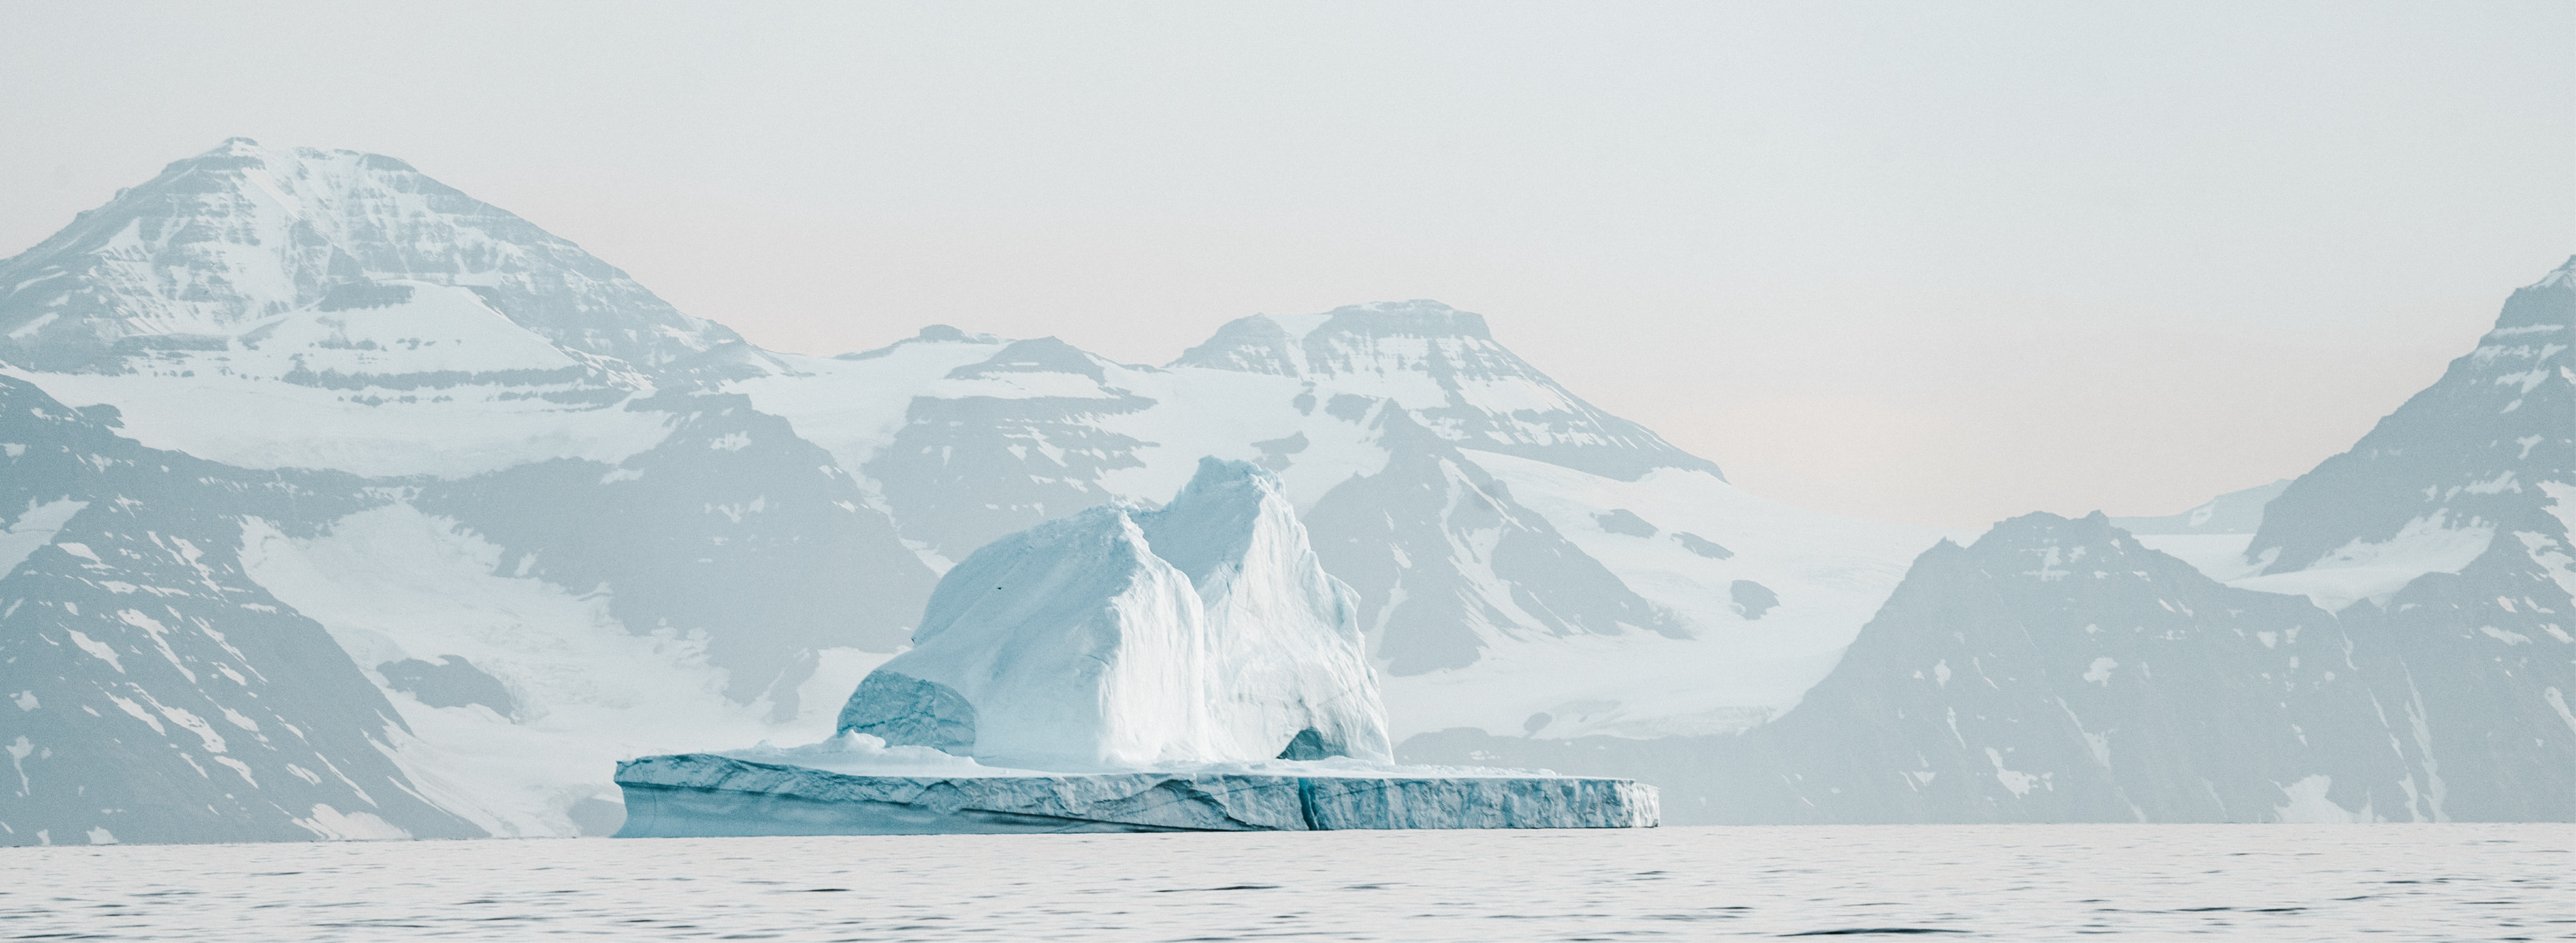
\includegraphics{banner1.png}

The \href{https://arcticdata.io/}{Arctic Data Center} is a place for researchers from around the world working in the Arctic to efficiently share, discover, access, and interpret complex data about the Arctic with less effort. Part of our mission is to provide hands on training at Arctic research conferences and in dedicated training sessions targeting Arctic researchers, especially early-career and under-represented populations. In 2020, we were able to support the development of undergraduate-level educational materials through our fellowship program. These materials are open source and available for reuse and/or modification either at the associated GitHub repository, the \href{http://training.arcticdata.io/}{Arctic Data Center Training page}, or the \href{https://dataoneorg.github.io/Education/}{DataOne Skillbuilding Hub}.

\includegraphics{adcfacts.png}

With over 5,700 datasets in the Arctic Data Center repository, these education modules are intended to equip students with the necessary tools and resources to unearth the story behind the data, one about one of the planet's fastest-changing ecosystems: the Arctic.

Encompassing Earth's northern most region, the Arctic is an icy sea surrounded by land characterized by a harsh climate with extreme variation in light and temperature. Diverse landscapes---from the sea ice to coastal wetlands, upland tundra, mountains, wide rivers, and the sea itself---support abundant wildlife and many cultures making the Arctic a region like no other in the world.

\textbf{However, what happens in the Arctic doesn't stay in the Arctic.}

The Arctic is warming twice as fast as the global average. The cause of such rapid warming is straightforward and well understood: It is human-caused climate change, and it is altering the relative amount of the Sun's energy that is absorbed, reflected, or radiated in the Arctic.

\includegraphics[width=0.7\textwidth,height=\textheight]{arcticsad.png}

According to \href{https://arctic.noaa.gov/Report-Card/Report-Card-2020}{15th annual NOAA Arctic Report Card}, the sea-ice extent in October of 2020 dropped to the lowest levels on record. Dramatic drops in Arctic ice like this are the main driver for rapid Arctic changes. Effects of a warming atmosphere on physical, chemical, biological, and human components of Arctic ecosystems are myriad, far-reaching, and accelerating. There is no facet of Arctic life that will remain untouched by the immensity of these changes.

Studying and understanding the Arctic is essential txo saving it, and ultimately ourselves. The Arctic Data Center repository is rich with real-world Arctic data just waiting to be explored. If you're ready to learn how, let's get started.

The National Wildlife Federation put together this \href{https://www.nwf.org/~/media/PDFs/Be\%20Out\%20There/Schoolyard\%20Habitats/ArcticEnvironment.pdf}{Activity Guide} if you'd like to learn more about the Arctic and climate change.

\hypertarget{intro}{%
\chapter*{\texorpdfstring{\textbf{Overview}}{Overview}}\label{intro}}
\addcontentsline{toc}{chapter}{\textbf{Overview}}

\includegraphics{banners2.png}

These datasets are intendented for reuse.

\textbf{Target Audience}: Undergraduate students

\textbf{Target Course(s)}: Ecology, biology, environmental sciences, resource management, statistics, data science, atmospheric sciences, GIS, sustainability, geology, sociology, chemistry, evolution, or similar

\textbf{Background knowledge needed}: None

\textbf{Prep Time}: 30 minutes

\textbf{Lesson Duration}: 2-3 hours

\textbf{Objectives}: By the end of this lesson, students will be able to\ldots{}.

\begin{itemize}
\tightlist
\item
  Understand what a data repository is and why it is used
\item
  Connect how data storage fits into the data life cycle
\item
  Become familiar with basic data collection methods and their affiliated file formats
\item
  Find and download data from the Arctic Data Center
\item
  Learn what metadata is and why it's important
\item
  Explain what open data is and why it is important for reproducibility
\end{itemize}

\textbf{Learned skills}:

\begin{itemize}
\tightlist
\item
  Finding the appropriate repository for different types of data and disciplines\\
\item
  Navigating a repository and understanding general data science terminology
\item
  Creating a data management plan
\end{itemize}

\textbf{Course Format}:

This module is meant to be taught within the timeframe of one lab period (or approximately 2 hours in length). Included in this lesson is an introductory video and prepared PowerPoint with time allotted for exploration into the Arctic Data Center's repository and completion of an in-class assignment. Instructors may want to assign students additional out of classwork, or use additional modules to round out a full unit.

\textbf{Suggested readings}: There are no required readings for this course, but feel free to recommend this introductory paper, ``\href{https://academic.oup.com/bioscience/article/67/6/546/3784601?login=true}{Skills and Knowledge for Data-Intensive Environmental Research}''.

\hypertarget{paleo}{%
\chapter*{Paleontology/Paleoecology}\label{paleo}}
\addcontentsline{toc}{chapter}{Paleontology/Paleoecology}

Paleontology is the study of the history of life on Earth as based on fossils. Fossils are the remains of plants, animals, fungi, bacteria, and single-celled living things that have been replaced by rock material or impressions of organisms preserved in rock.

Paleoecology is the study of interactions between once-living organisms and their environmental surroundings. Interactions between organisms can take a variety of forms, including competition between similar organisms for resources, predation of one organism by another, and symbiosis between different organisms to enable each organism to survive and reproduce. Read more \href{https://www.digitalatlasofancientlife.org/learn/paleoecology/}{here}.

\hypertarget{my-section}{%
\section*{Using sediment core data to better understand the wooly mammoth extinction}\label{my-section}}
\addcontentsline{toc}{section}{Using sediment core data to better understand the wooly mammoth extinction}

\includegraphics{images/mammoths.png}

\textbf{The Dataset in Question}

\href{https://arcticdata.io/catalog/view/doi\%3A10.18739\%2FA24746R6K}{Sediment core data related to the extinction of Mammuthus primigenius, St.~Paul Island, Alaska, 2014.}

This dataset is brought to you by \href{https://www.uaf.edu/cfos/people/faculty/detail/matthew-wooller.php}{Matthew Wooller} (he/him/his), an interdisciplinary scientist, applying stable isotope techniques to understand the influence of changing environmental conditions on past and present ecosystems.

The full paper associated with this dataset is avalible \href{https://www.pnas.org/content/113/33/9310}{here}.

\textbf{The Story}

Relict woolly mammoth (Mammuthus primigenius) populations survived on several small Beringian islands for thousands of years after mainland populations went extinct.

\textbf{What We Know}

Five independent indicators of extinction show that mammoths survived on St.~Paul until 5,600 ± 100 years ago. Vegetation composition remained stable during the extinction window, and there is \emph{no evidence} of human presence on the island before 1787 CE, suggesting tha=t these factors were not extinction drivers.

\textbf{The Data Says}

Instead, the extinction coincided with declining freshwater resources and drier climates between 7,850 and 5,600 years ago, as inferred from sedimen-tary magnetic susceptibility, oxygen isotopes, and diatom and cla-doceran assemblages in a sediment core from a freshwater lake on the island, and stable nitrogen isotopes from mammoth remains.

Contrary to other extinction models for the St.~Paul mammoth population , this evidence indicates that this mammoth population died out because of the synergistic effects of shrinking island area and freshwater scarcity caused by rising sea levels and regional climate change. Degradation of water quality by intensified mammoth activity around the lake likely exacerbated the situation. The St.~Paul mammoth demise is now one of the best-dated prehistoric extinctions, highlighting freshwater limitation as an overlooked extinction driver and underscoring the vulnerability of small island populations to environmental change, even in the absence of human influence.

\includegraphics[width=0.7\textwidth,height=\textheight]{images/woolydata.png}

\emph{Paleoenvironmental proxies at Lake Hill, plotted against time. Shown are relative abundances of planktonic (blue bars), tychoplanktonic (maroon bars), and high-conductivity--tolerant diatoms (orange bars); ratio of pelagic and littoral cladocerans (gray curve); relative abundance (\%) of cladoceran Alona circumfibriata, which is tolerant of high lake water conductivity (purple bars); δ 18 O values from aquatic invertebrate chitin (blue curve); δ 15 N values from mammoth collagen (red curve); sediment magnetic susceptibility (in AU); and accumulation rates for herb and shrub pollen types (light green and tan curves, respectively). The estimated timing of extinction (yellow vertical bar) and the magnetic susceptibility curve are included to help establish the stratigraphic correlation between Figs. 2 and 3. }

\hypertarget{flowers}{%
\chapter*{Oceanography}\label{flowers}}
\addcontentsline{toc}{chapter}{Oceanography}

The Arctic Ocean is, on average, the shallowest of Earth's oceans. Its vast continental shelf areas, which account for approximately half of the Arctic Ocean's total area, are heavily influenced by the surrounding land masses through river run-off and coastal erosion. As a main area of deep water formation, the Arctic is one of the main «engines» of global ocean circulation, due to large freshwater inputs, it is also strongly stratified. The Arctic Ocean's complex oceanographic configuration is tightly linked to the atmosphere, the land, and the cryosphere. The physical dynamics not only drive important climate and global circulation patterns, but also control biogeochemical cycles and ecosystem dynamics. Current changes in Arctic sea-ice thickness and distribution, air and water temperatures, and water column stability are resulting in measurable shifts in the properties and functioning of the ocean and its ecosystems. The Arctic Ocean is forecast to shift to a seasonally ice-free ocean resulting in changes to physical, chemical, and biological processes. These include the exchange of gases across the atmosphere-ocean interface, the wind-driven ciruclation and mixing regimes, light and nutrient availability for primary production, food web dynamics, and export of material to the deep ocean. In anticipation of these changes, extending our knowledge of the present Arctic oceanography and these complex changes has never been more urgent.

\hypertarget{section}{%
\section*{Frost flowers on young Arctic sea ice}\label{section}}
\addcontentsline{toc}{section}{Frost flowers on young Arctic sea ice}

\includegraphics{images/frostflowers.jpg}

\textbf{The Data}

\href{https://arcticdata.io/catalog/view/doi\%3A10.18739\%2FA2N036}{Frost flowers on young Arctic sea ice: The climatic, chemical and microbial significance of an emerging ice type}

This dataset is brought to you by \href{https://www.ocean.washington.edu/story/Jody_Deming_Ecosystem}{Jody W. Deming} (she/her), an American oceanographer. She is a professor of Oceanography and a marine microbiologist at the University of Washington. Her research interests include studies of cold adapted microbes in their relation to astrobiology, biotechnology, and bioremediation.

The full paper associated with this dataset is avalible \href{https://agupubs.onlinelibrary.wiley.com/doi/full/10.1002/2014JD021736}{here}.

\textbf{What We Know}

Frost flowers are highly saline ice structures that grow on the surface of young sea ice, a spatially extensive environment of increasing importance in the Arctic Ocean. Although frost flower blooms are frequently observed in both polar oceans, little is understood about the physical, chemical and biological nature of these structures. To investigate their microbiology Bowman and Deming learned to grow frost flowers in a freezer lab at the University of Washington before moving their study into the field, collecting frost flowers during several challenging expeditions. With these first samples they have begun to develop the concept of frost flowers as a microbial habitat. Their goal is to probe the secrets of microbial life in very cold environments, a priority of the astrobiology community. Since many of the planets and moons in our solar system that might harbor life are very cold and covered in ice, determining the habitability of these planets and moons requires an understanding of the limits of life (as we know it) in the very coldest environments on Earth.

\textbf{What we found out}

Bowman and Deming have discovered that bacteria are consistently more abundant in frost flowers than in sea ice. Since microscopic pockets in sea ice are known to support an active community of psychrophiles (cold-loving microorganisms), even in the coldest months of the year, these results are encouraging. Frost flowers, however, are much colder than sea ice. In their last field season at Barrow, Alaska, working between intense blizzards blowing off the Beaufort Sea, they collected frost flowers and underlying sea ice for a comparative analysis of the life they host. Techniques designed to identify weakly respiring organisms are being employed in one of the coldest natural environments studied so far.

\includegraphics{images/flowersdata.png}

Finally, while frost flowers are too harsh an environment for most life, they may have ironically played a role in the origin of life on Earth. Formaldehyde, found in high concentrations in some frost flowers, is useful for making simple sugars including ribose. Ribose is an essential component of RNA, a molecule used to temporarily encode genetic information by every cell on Earth. Although today DNA is the primary molecule for passing on genetic information from one generation to the next, RNA may have been the first molecule to do so. On the early Earth frost flowers could have contributed ribose to a global ``primordial soup'' of molecules that allowed the first genetic system to form. Investigating this hypothesis is a particular challenge, as simple sugars are quickly consumed by ubiquitous and omnipresent microbes in today's natural environment. To continue this line of research, Bowman and Deming are building a special chamber to grow frost flowers under ultra-clean conditions.

\hypertarget{ecology}{%
\chapter*{Ecology}\label{ecology}}
\addcontentsline{toc}{chapter}{Ecology}

Ecology is the study of how organisms interact with one another and with their physical environment. The distribution and abundance of organisms on Earth is shaped by both biotic, living-organism-related, and abiotic, nonliving or physical, factors. Ecology is studied at many levels, including organism, population, community, ecosystem, and biosphere. Read more \href{https://www.khanacademy.org/science/biology/ecology/intro-to-ecology/a/what-is-ecology}{here}.

\hypertarget{this-section}{%
\section*{Labeling study of water use by tundra evergreens in the winter spring transition}\label{this-section}}
\addcontentsline{toc}{section}{Labeling study of water use by tundra evergreens in the winter spring transition}

\includegraphics{evergreen.jpg}

\textbf{The Data}

\href{https://arcticdata.io/catalog/view/doi\%3A10.18739\%2FA22V2CB1P}{Labeling study of water use by tundra evergreens in the winter spring transition}

This dataset is brought to you by \href{http://faculty.fiu.edu/~oberbaue/}{Steven F. Oberbauer} (he/him), a Professor of Biological Sciences at Florida International University. His area of interests are plant and ecosystem physiology, energy balance, plant phenology and productivity of vascular plants and bryophytes, particularly in response to climate change.

The full paper associated with this dataset is avalible \href{https://bsapubs.onlinelibrary.wiley.com/doi/full/10.3732/ajb.1500358}{here}.

\textbf{What We Know}

The cold season in the Arctic extends over 8 to 9 mo, yet little is known about vascular plant physiology during this period. Evergreen species photosynthesize under the snow, implying that they are exchanging water with the atmosphere. However, liquid water available for plant uptake may be limited at this time.

\textbf{What we found out}

Evergreen tundra plants take up water under snow cover, some via roots, but also likely by foliar uptake. The ability to take up water in the subnivean environment allows evergreen tundra plants to take advantage of mild spring conditions under the snow and replenish carbon lost by winter respiration.

\hypertarget{greenland}{%
\chapter*{Arctic Happenings}\label{greenland}}
\addcontentsline{toc}{chapter}{Arctic Happenings}

\hypertarget{section-id}{%
\section*{Global Impacts of the Melting Greenland Ice Sheet and Melting Sea Ice}\label{section-id}}
\addcontentsline{toc}{section}{Global Impacts of the Melting Greenland Ice Sheet and Melting Sea Ice}

\includegraphics{images/greenlandmelt.jpg}

\textbf{Inside this Module}

\href{https://arcticdata.io/catalog/view/doi\%3A10.18739\%2FA2TM7216N}{Arctic Happenings - Global Impacts of the Melting Greenland Ice Sheet and Melting Sea Ice, 1961-2015.}

\href{https://ahrl.rutgers.edu/greenland-lessons}{Arctic Happenings} is part of a four-part educational module designed for upper middle school, high school and undergraduate students. All the digital materials for this module are freely available online and include rich video and data resources plus step-by-step instructions.

These materials were created by Missy Holzer, Ph.D., Asa Rennermalm, Ph.D..

\bibliography{book.bib,packages.bib}

\end{document}
